\documentclass[12pt]{article}
\usepackage{paper,math}
\usepackage[margin=1in]{geometry}
\addbibresource{references.bib}

\title{Genomorientierte Bioinformatik \\ - \\ Differential Analysis}
\author{Malte Weyrich}
\date{\today}
% Conditionally display thoughts (hide by switching to `\boolfalse`)
% \booltrue{INCLUDECOMMENTS}
\newcommand{\malte}[1]{\coauthorComment[Malte]{#1}}

\begin{document}

% Title Page -------------------------------------------------------------------
\maketitle
\begin{abstract}
\textit{Alternatives Splei\ss ing} ist ein fundamentaler zellulärer Mechanismus  mit 
gro\ss en Einfluss auf regulatorische Prozesse und Genprodukte.
Dabei werden die \textit{Exons} eines Transkripts teilweise übersprungen oder neu angeordnet. 
Verantwortlich für diesen Prozess ist das \textit{Splei\ss osom}. 
Im Folgenden wird ein Programm zur Quantifizierung von \textit{Skipped Exon Events} vorgestellt und
dessen Ergebnisse mit einem Hypothesen Test evaluiert. 
Es wurde auf zehn \textit{bam}-Dateien ausgeführt mit \textit{annotation\_b37.gtf}
als Referenzgenom.
Zusätzlich werden die Resultate mit einem bereist publizierten Tool (\textit{\textbf{DEXSeq}} aus \cite{anders2012detecting}) verglichen.

\end{abstract}

\newpage

\tableofcontents

\newpage

% Paper ------------------------------------------------------------------------

% ------------------------------------------------------------------------------
\section{Berechnung der Percent Spliced-In Werte}
\subsection{Definition}\label{sec:Definition}
\textit{Percent Spliced-In (PSI)} Werte werden in der Bioinformatik genutzt, um die 
Evidenz von \textit{Skipped Exon Events} anhand von beobachteten Daten darzustellen. 
Die \textit{Skipped Exon Events} entstehen durch \textit{Alternatives Splei\ss en} und beeinflussen ma\ss geblich das Proteinendprodukt
eines \textit{Gens}.
Die Expression von Transkripten kann mittels \textit{RNAseq} untersucht werden, bei dem die Sequenzen der
vorliegenden Transkripte sequenziert werden.
Somit entstehen Milliarden von \textit{Reads}, welche 
mit der Hilfe von \textit{Software} zurück auf das \textit{Referenz Genom} projiziert werden können.
Anschlie\ss end werden die \textit{Reads} annotiert, das hei\ss t es wird geschaut, von 
welchen Transkripten die \textit{Reads} stammen. 
Der \textit{PSI} Wert wird dann mittels \textit{Inclusion Read Counts (\textbf{IRC})} und \textit{Exclusion Read Counts (\textbf{ERC})} berechnet werden:

\[
    PSI := \frac{IRC}{IRC + ERC}
.\]
Sei $G$ ein \textit{Gen}  mit Transkripten $WT$ und $SV$. 
Zudem sei $se$ eine, durch die Annotation implizierte, übersprungene Region in $WT$, 
für die der \textit{PSI} Wert berechnet werden soll.
Wenn $R$ die Menge an aligniernten \textit{Read Pairs} auf $G$ ist,
dann ist $I \subseteq R$ die Menge an alignierten \textit{Read Pairs} auf $se$ und somit 
\[
   IRC_{se} := \left|I\right|
.\]
Die \textit{Exclusion Reads} $E \subseteq R$ sind genau die \textit{Read Pairs},
welche nicht auf $se$ \textit{gemapped}  werden können.

\[
   ERC_{se} := \left|E\right|
.\]
Ein \textit{PSI} Wert von 1 würde beispielsweise bedeuten, dass die Region $se$ in den
beobachteten Transkripten eines \textit{Gens} überwiegend inkludiert wurde
(also nicht durch das \textit{Splei\ss osom} heraus gesplie\ss t wurde), während ein Wert von 0
auf ein vermehrtes Ausschlie\ss en von $se$ hindeuten würde.


\subsection{Programm Logik}
\begin{figure}[htbp]
    \centering
    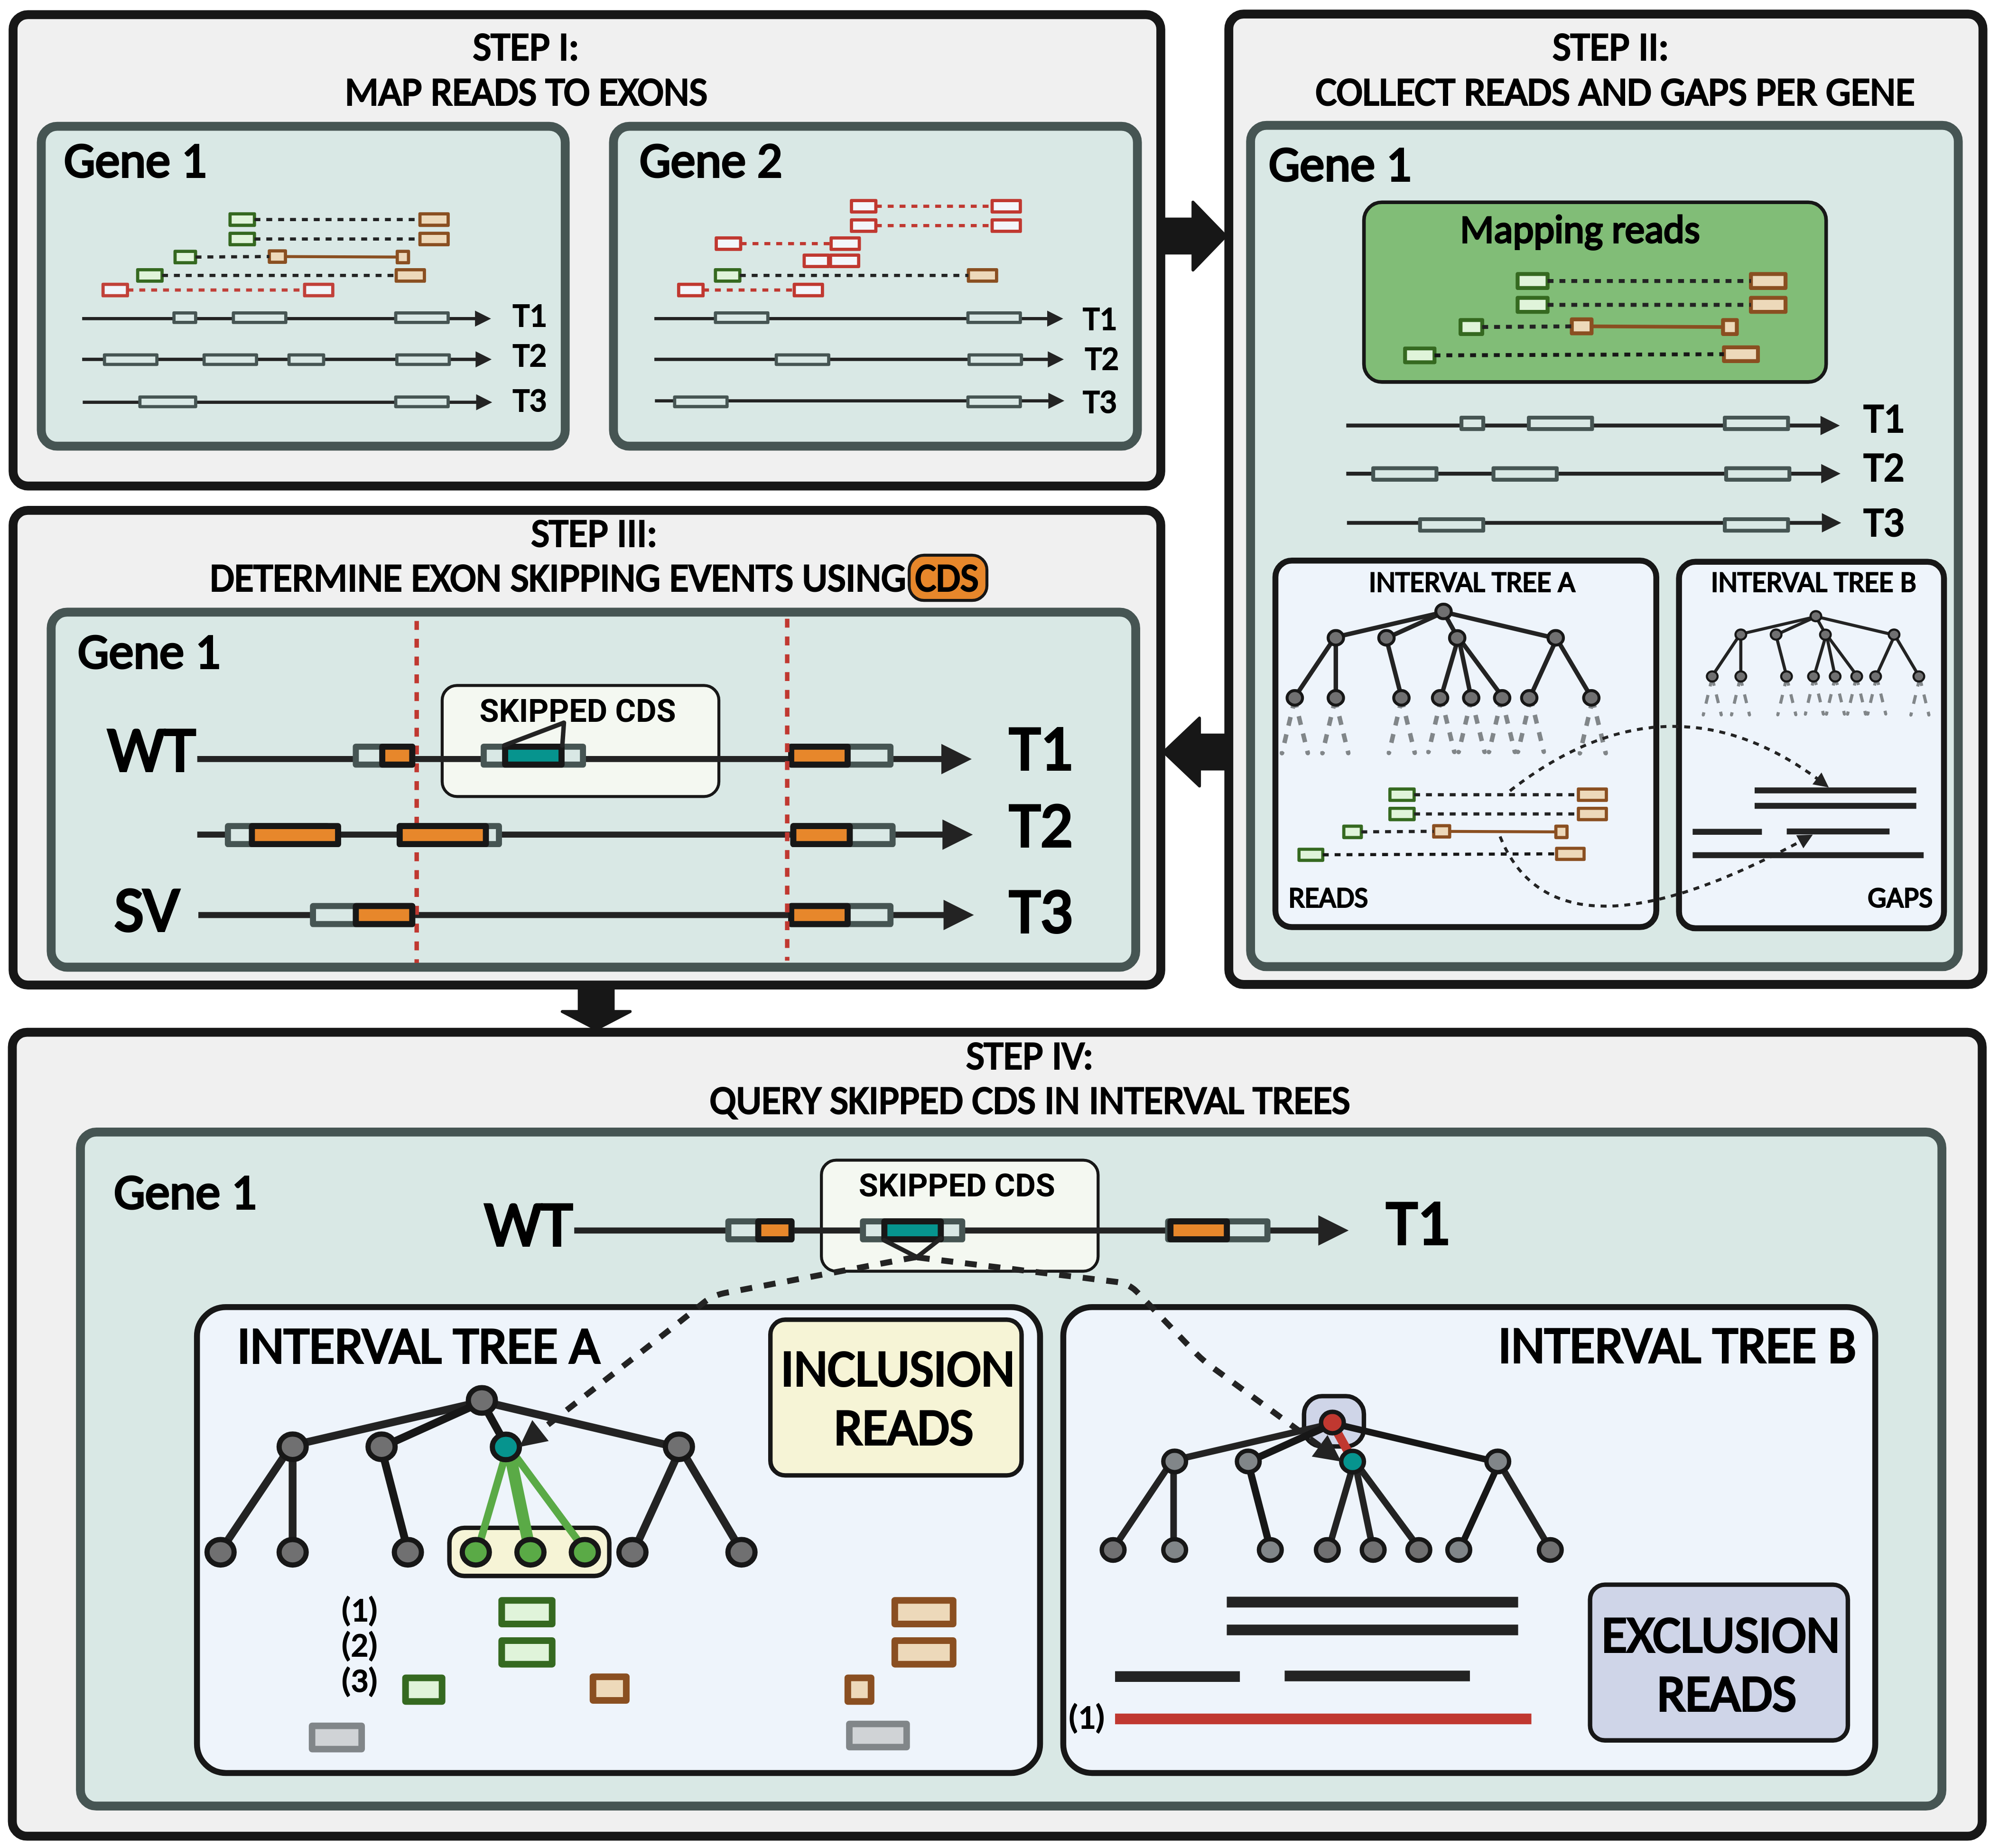
\includegraphics[width=0.99\textwidth]{./figures/PSI-Mapping.png}
    \caption{Programmlogik zur Berechnung der \textit{IRC} und \textit{ERC counts} pro \textit{Skipped Exon Event}.
    In dem Beispiel hätte das übersprungene Exon von \textbf{G1} einen \textit{PSI} Wert von 0.75.
    Die Abbildung wurde mit \cite{biorender} erstellt.}

    \label{fig:PSI-Mapping-png}
\end{figure}

Der \textit{JAR} werden eine \textit{bam}- und ein \textit{GTF}-Datei übergeben.
Zudem muss eine Ausgabedatei Spezifiziert werden:
\begin{verbatim*}
    java -jar psi.jar -bam <bam> 
                      -gtf <gtf> 
                      -o <ausgabe.psi>
\end{verbatim*}

Die \textit{JAR} liest zunächst die \textit{GTF}-Datei ein und speichert alle \textit{Gene} und deren annotierte
\textit{Transkripte} ab. 
Dabei enthält jedes \textit{Transkript} jeweils dessen \textit{Exons} \textbf{und} \textit{Coding DNA Sequences (CDS)}.
Gleichzeitig wird die \textit{bam}-Datei mittels der \textit{samtools library} decodiert und abgespeichert.
Nach der Einleseroutine kann das Programm in vier Schritte eingeteilt werden (siehe Abbildung \ref{fig:PSI-Mapping-png}):

\begin{itemize}
    \item[\textbf{I.}] \textbf{MAP READS TO EXONS}

        Die \textit{Read Pair} Koordinaten werden mit den \textit{\textbf{Exon}} Koordinaten der Transkripte abgeglichen. 
        Sobald mindestens ein \textit{Read Pair} auf ein \textit{Gen} \textit{mapped}, wird das \textit{Gen}
        in einer \textit{ArrayList<Gene> \textbf{mappedGenes}} abgelegt.
        Die Kriterien für einen validen \textit{Read} wurden bereits im letzten Report geklärt. 
        Es werden nur \textit{Reads} in \textit{mappedGenes} hinzugefügt, wenn sie auf genau ein einziges \textit{Transkript}
        passen.

    \item[\textbf{II.}] \textbf{COLLECT READS AND GAPS PER GENE}

        Für jedes der Gene in \textbf{\textit{mappedGenes}} werden nun zwei Intervallbäume $A, B$ erstellt.
        Baum $A$ beinhaltet alle \textit{AlignmentBlocks} der zum Gen zugeteilten \textit{Read Pairs},
        während Baum $B$ die Lücken zwischen einzelnen \textit{AlignmentBlocks} und zwischen
        den \textit{Forward} und \textit{Reverse Reads} abspeichert.

    \item[\textbf{III.}] \textbf{DETERMINE EXON SKIPPING EVENTS USING CDS}

        Im nächsten Schritt wird über alle Gene aus \textbf{\textit{mappedGenes}} iteriert.
        Für jedes einzelne Gen werden alle \textit{Skipped Exon Events} mittels der
        \textit{CDS} des Gens berechnet. Dabei wird dieselbe Logik wie in 
        Report 1 verwendet.

    \item[\textbf{IV.}] \textbf{QUERY SKIPPED CDS IN INTERVALTREE}

        Für jede \textit{CDS} werden nun dessen Intervalle in den Bäumen $A, B$ abgefragt und die
        \textit{Read IDs} gezählt.
        \[
        IRC := |\left\{\textit{A.\textbf{getIntervalsSpannedBy}(CDS.getStart(), CDS.getStop())}\right\}|
        \]
        \[
        ERC := |\left\{\textit{B.\textbf{getIntervalsSpanning}(CDS.getStart(), CDS.getStop())}\right\}|
        \]
        Dabei werden für $IRC$ \textbf{Intervalle} in $A$ betrachtet, \textbf{die von der \textit{CDS} überspannt werden} \\
        ($\equiv$ "\textit{Reads} die innerhalb der \textit{CDS} liegen") und für 
        $ERC$ werden \textbf{Intervalle} in $B$ gesucht, \textbf{die die \textit{CDS} überspannen} 
        ($\equiv$ "Intervalle, die die \textit{CDS} beinhalten").
\end{itemize}
\newpage

Die \textit{PSI} Werte werden in die Ausgabedatei mit folgendem Format geschrieben:
\begin{verbatim*}
   Gene ID            cdsStart-cdsStop   IRC   ERC  Total  PSI
   ENSG00000165623.5  13275735-13275801  25    13   38     0.65
   ...                ...                ...   ...  ...    ...
\end{verbatim*}

\section{Hypothesen Test}
Wir wollen untersuchen, ob der Prozess des \textit{Alternativen Splei\ss ens} anhand von 
\textit{Exon Skipping Events} ($\mathbf{\Psi}$) rein zufällig stattfindet, oder von regulatorischen 
Mechanismen gesteuert wird. 

\begin{itemize}
    \item \textbf{H\textsubscript{0}} := \textit{Exon Skipping Events} finden zufällig statt.
    \item \textbf{H\textsubscript{1}} := \textit{Exon Skipping Events} sind nicht reiner Zufall.
\end{itemize}
Dafür nehmen wir an, dass die Anzahl an \textit{IRC} Binomial Verteilt ist:

\[
P(i,N|p) = \binom{N}{i}p^{i}(1-p)^{N-i}
.\]
Hierbei beschreibt $p$ die Wahrscheinlichkeit, dass ein einzelnes \textit{Exon} als \textit{Inclusion Read} klassifiziert wird,
während $N$ die Anzahl an \textit{Reads} darstellt, die für das momentane \textit{Exon} einen Informationsgehalt haben.
Zudem gehen wir davon aus, dass jedes Transkript mindestens einen informativen \textit{Read} pro Exon hat.

Für den Test wurden die zehn Ausgabedateien der \textit{JAR} in zwei Gruppen unterteilt (siehe Tabelle \ref{tab:einteilung}):

\begin{table}[htpb]
    \centering
    \caption{Einteilung der Samples in zwei Gruppen}
    \label{tab:einteilung}
\begin{tabular}{|l||c|c|c|c|c|c|c|c|c|c|} \hline
     Ausgabedatei $i$   & 1 & 2 & 3 & 4 & 5 & 6 & 7 & 8 & 9 & 10 \\\hline
     Gruppe $g_{i}$ & 1 & 1 & 1 & 1 & 1 & 2 & 2 & 2 & 2 & 2 \\\hline
     IRC          &$i_{1}$&$i_{2}$&$i_{3}$&$i_{4}$&$i_{5}$&$i_{6}$&$i_{7}$&$i_{8}$&$i_{9}$&$i_{10}$  \\\hline
     Gesamt Anzahl&$N_{1}$&$N_{2}$&$N_{3}$&$N_{4}$&$N_{5}$&$N_{6}$&$N_{7}$&$N_{8}$&$N_{9}$&$N_{10}$  \\ \hline\hline
     $\mathbf{\Psi_{reduced}} \sim (p_{0})$   &$p_{0}$&$p_{0}$&$p_{0}$&$p_{0}$&$p_{0}$&$p_{0}$&$p_{0}$&$p_{0}$&$p_{0}$&$p_{0}$\\\hline
     $\mathbf{\Psi_{full}} \sim  (p_{1}, p_{2})$ &$p_{1}$&$p_{1}$&$p_{1}$&$p_{1}$&$p_{1}$&$p_{2}$&$p_{2}$&$p_{2}$&$p_{2}$&$p_{2}$\\\hline
\end{tabular}
\end{table}
\newpage

Dabei simulieren wir zwei \textit{Modellen}:
\begin{itemize}
    \item $\mathbf{\Psi_{reduced}} \sim(p_{0})$: Hat einen einzigen Parameter $p_{0}$ für alle Gruppen.
    \item $\mathbf{\Psi_{full}} \sim(p_{1}, p_{2})$: Besitzt zwei verschiedenen Parameter.
\end{itemize}
Die \textit{Likelihood} kann nun mit der \textit{Maximum Likelihood Estimation} Methode
abgeschätzt werden.
Die \textit{Log-Likelihood Funktionen} lasses sich wie folgt definieren:
\begin{itemize}
\item $\mathbf{\mathcal{L}_{reduced}}(p_{0}) := \log\Big(\prod_{j = 1}^{10}P(i_{j},N_{j}|p_{0})\Big)$
\item $\mathbf{\mathcal{L}_{full}}(p_{1}, p_{2}) := \log\Big(\prod_{j = 1}^{10}P(i_{j},N_{j}|p_{g_{j}})\Big)$
\end{itemize}
Indem man die jeweilige Ableitung von $\mathbf{\mathcal{L}}$ gleich null setzt, 
erhält man die \textit{MLE} Schätzer $\hat p_{0}$ und $\hat p_{1}, \hat p_{2}$:
\begin{align*}
    \mathbf{\mathcal{L}}(\hat p_{0})  &= \log\Bigg( \prod_{j=1}^{10} \binom{N}{i_{j}}p_{0}^{i_{j}}(1-p_{0})^{N_{j}-i_{j}}  \Bigg)\\
    \mathbf{\mathcal{L}}(\hat p_{0})  &= \sum_{j=i}^{10} \log\Bigg(\binom{N_{j}}{i_{j}}\Bigg) + \log(p_{0})\sum_{j=1}^{10} i_{j} + \log(1-p_{0}) \sum_{j=1}^{10} (N_{j} - i_{j}) \\
    \mathbf{\mathcal{L}}'(\hat p_{0}) &= \frac{\sum_{j=1}^{10} i_{j}}{p_{0}} - \frac{\sum_{j=1}^{10} (N_{j} - i_{j})}{1-p_{0}} \\
                   0 &= \frac{\sum_{j=1}^{10} i_{j}}{p_{0}} - \frac{\sum_{j=1}^{10} (N_{j} - i_{j})}{1-p_{0}} \\
                   \hat p_{0} &= \frac{\sum_{j=1}^{10} i_{j}}{\sum_{j=1}^{10} N_{j}} \\ 
                              & \\
    \mathbf{\mathcal{L}}(\hat p_{1}, \hat p_{2})  &= \log\Bigg( \prod_{j=1}^{10} \binom{N}{i_{j}}p_{g_{i}}^{i_{j}}(1-p_{g_{i}})^{N_{j}-i_{j}}  \Bigg)\\
    % \mathbf{\mathcal{L}}(\hat p_{1}, \hat p_{2}) &= \sum_{j \in Gruppe_{1}} \log\Bigg(\binom{N_{j}}{i_{j}}\Bigg) + \log(p_{1})\sum_{j \in Gruppe_{1}} i_{j} + \log(1-p_{1}) \sum_{j \in Gruppe_{1}} (N_{j} - i_{j}) \\ 
    %                                              &\hspace{6mm} + \sum_{j \in Gruppe_{2}} \log\Bigg(\binom{N_{j}}{i_{j}}\Bigg) + \log(p_{2})\sum_{j \in Gruppe_{2}} i_{j} + \log(1-p_{2}) \sum_{j \in Gruppe_{2}} (N_{j} - i_{j}) \\ 
    \iff \mathbf{\mathcal{L}}(\hat p_{1}, \hat p_{2}) &= \mathbf{\mathcal{L}_{Gruppe_{1}}}(p_{1}) + \mathbf{\mathcal{L}_{Gruppe_{2}}}(p_{2}) \\
    \mathbf{\mathcal{L}_{Gruppe_{1}}}'(\hat p_{1}) &= \frac{\sum_{j \in Gruppe_{1}}i_{j}}{p_{1}} - \frac{\sum_{j \in Gruppe_{1}} (N_{j} - i_{j})}{1-p_{1}} \\
    \iff \hat p_{1} &= \frac{\sum_{j \in Gruppe_{1}} i_{j}}{\sum_{j \in Gruppe_{1}} N_{j}}\\
    \mathbf{\mathcal{L}_{Gruppe_{2}}}'(\hat p_{2}) &= \dots \\
    \hat p_{2} &= \frac{\sum_{j \in Gruppe_{2}} i_{j}}{\sum_{j \in Gruppe_{2}} N_{j}}\\
\end{align*}

Die \textit{Likelihood Schätzer} können nun verwendet werde, um $\mathbf{\mathcal{L}_{reduced}}(\hat p_{0})$ und $\mathbf{\mathcal{L}_{full}}(\hat p_{1}, \hat p_{2})$ zu 
berechnen. Zudem bestimmen wir jeweils die \textit{Likelihood Ratio Statistik (LRS)}:
\[
    LRS := -2 \log\Big(\frac{\mathcal{L}_{reduced}}{\mathcal{L}_{full}}\Big)
.\]

Dabei gilt: 
\[
    LRS \sim \chi^{2}
.\]
Somit können wir für jeden der berechneten \textit{PSI} Werte einen $p$ Wert berechnen. 
Zudem wurde die \textit{Benjamini Hochburg} Methode (\cite{bh_correction}) verwendet, um die $p$ Werte 
anzupassen, da multiple Hypothesen Tests durchgeführt wurden.

Das \textit{R} Skript \textit{LRS.R} implementiert die Berechnung der \textit{LRS} und $p$
Werte und schreibt die Resultate in eine Ausgabedatei:

\begin{verbatim*}
gene  exon        p0    p1    p2      llreduced    llfull   lrs  pvalue padj
id    start-stop  0.64  0.64  0.65  -25.86       -25.82  0.07 0.78   0.9
...   ...         ...   ...   ...   ...          ...     ...  ...    ...
    
\end{verbatim*}

\section{Komplexität und Korrektheit}\label{sec:Komplexität und Korrektheit}
\subsection{Komplexität}\label{sec:Komplexität}
Das entwickelte Java Programm benutzt für das Einlesen der \textit{GTF}-Datei, dem Bestimmen
der \textit{Exon Skipping Events} und dem \textit{Mapping} der \textit{Reads} dieselbe Komplexität
wie die Programme aus Report 1 und 3.
Das einzige was an zusätzlichem Aufwand anfällt ist die Erstellung der Intervallbäume pro Gen (A) und das 
anschlie\ss ende Zählen der \textit{IRC} und \textit{ERC} (B).
\begin{itemize}
    \item[\textbf{(A)}] \textbf{Erstellen der Intervallbäume:} 

        Sei $\tilde G$ die Menge aller \textit{Gene} aus der vorliegenden \textit{Annotation} und
        $\tilde R$ die Menge aller \textit{Reads} aus dem Sequenzierexperiment.
        Dann ist $G \subseteq \tilde G$ die Teilmenge an \textit{Genen}, auf 
        welche es ein \textit{Mapping} von \textit{Reads} gibt.
        Jedes \textit{Gen} $g_{i} \in  G$ hat also eine Teilmenge $R_{i}$ an
        alignierten \textit{Reads} aus $\tilde R$.
        Für jedes Gen $g_{i}$ werden alle zugehörigen \textit{Reads} $R_{g}$
        in die Intervallbäume $A$ und $B$ eingefügt.
        Das Einfügen in einen Intervallbaum hat ein logarithmisches 
        Kostenma\ss : $\mathcal{O}(\log n)$, wobei $n$ die Gesamtanzahl an
        Intervallen ist, welche sich bereits in dem Baum befinden.
        Für das konsekutive Einfügen von \textit{Reads} aus $R_{g}$ in $A$ ergibt sich folgende, von 
        oben abgeschätzte Laufzeit:
        \begin{align*}
            1  + \log(1) + \log(2) + \dots + \log(|R_{g}| - 1) &< \sum^{|R_{g}|} \log (|R_{g}|) \\
                                                               &\in \mathcal{O}\Big(|R_{g}| \cdot \log(|R_{g}|)\Big)
        \end{align*}

        Das gleiche gilt für die \textit{Gaps}, welche in den zweiten Intervallbaum eingefügt werden:
        \begin{align*}
        1  + \log(1) + \log(2) + \dots + \log(R_{i}/2 + c) &< \sum^{|R_{g}|/2 + c} \log (|R_{g}|/2 + c) \\
                                                           &\in \mathcal{O}\Big((|R_{g}|/2 +c) \cdot \log(|R_{g}|/2 + c)\Big) \\
                                                           &\in \mathcal{O}\Big((|R_{g}| + c) \cdot \log(|R_{g}| + c)\Big)
        \end{align*}
        Da es sich um \textit{paired end} Daten handelt (Abbildung \ref{fig:PSI-Mapping-png}), gibt es zwischen jedem \textit{Read Pair} einen \textit{Gap}
        (also insgesamt $|R_{g}|/2$) und zusätzlich $c$ viele \textit{Gaps} zwischen den jeweiligen
        \textit{AlignmentBlocks} der \textit{Reads}.

        Da wir insgesamt $|G|$ viele Gene haben also:
        \[
            \mathcal{O}\Bigg(|G| \cdot \Big(|R_{\tilde g}| \cdot \log(|R_{\tilde g}|) + (|R_{\tilde g}|+c) \cdot \log(|R_{\tilde g}| + c)\Big)\Bigg)
        \]
        , wobei 
        \[
            \tilde g := \operatornamewithlimits\forall_{R_{g} \in R, R_{g} \not =  R_{\tilde g}} R_{g} \le R_{\tilde g}
        \]
        das Gen mit den meisten alignierten \textit{Reads} ist.

    \item[\textbf{(B)}] \textbf{Ermittlung der \textit{IRC} und \textit{ERC:}}

        Eine Suchoperation in einem Intervallbaum hat ebenfalls eine Komplexität von $\mathcal{O}(\log n)$.
        Nach \textbf{Schritt (A)} befinden sich in den Bäumen $A,B$ von einem Gen $g \in G$ genau $|R_{i}|$
        und $|R_{i}|/2 + c$ viele \textit{Reads}.
        Jedes $g \in G$ besitzt $e_{g}$ viele \textit{Exon Skipping Events}. So muss 
        $|e_{g}|$ oft in jeweils beiden Bäumen eine Suche getätigt werden.
        Pro Gen also:
        \[
            |e_{g}| \cdot \log(R_{\tilde g}) + |e_{g}| \cdot \log(R_{\tilde g}/2 + c) = |e_{g}| \cdot  (\log(R_{\tilde g}) + \log(R_{\tilde g} + c) \in \mathcal{O}\Big(|e_{g}| \cdot \log(R_{\tilde g} + c)\Big)
        .\]
\end{itemize}
\subsection{Korrektheit}\label{sec:Korrektheit}
Der Ansatz mit den Intervallbäumen ist Korrekt. In den Intervallbäumen werden nur \textit{Reads} abgespeichert, die genau auf
ein \textit{Transkript} passen. Somit werden schon mal alle \textit{Reads} ohne eindeutigen Informationsgehalt 
ignoriert. Zusätzlich werden zu jeder hinzugefügten Region (in beiden Bäumen), die \textit{Ursprungs ID}
(in diesem Fall die Transkript ID) und die \textit{Read ID} gespeichert. 
Da der Intervallbaum korrekt implementiert ist, liefert diese entweder alle 
Intervalle, die von der übersprungenen \textit{CDS} beinhaltet werden (Baum $A$),
oder alle \textit{Gaps}, welche die \textit{CDS} überspannen (Baum $B$).
Die Anzahl an einzigartigen \textit{Read IDs} beider Abfragen ergibt dann die 
jeweiligen \textit{IRC} und \textit{ERC}.
Der einzige Sonderfall ergibt sich, wenn eine Region $r$ aus dem Baum $B$ dieselbe
\textit{Transkript ID} hat wie das der übersprungenen \textit{CDS}. 
In diesem Fall impliziert $r$ dann keinen \textit{ERC} sonder einen \textit{IRC}, 
denn $r$ wurde schlie\ss lich eindeutig auf das \textit{Transkript} der \textit{CDS}
aligniert.
\begin{figure}[htpb]
    \centering
    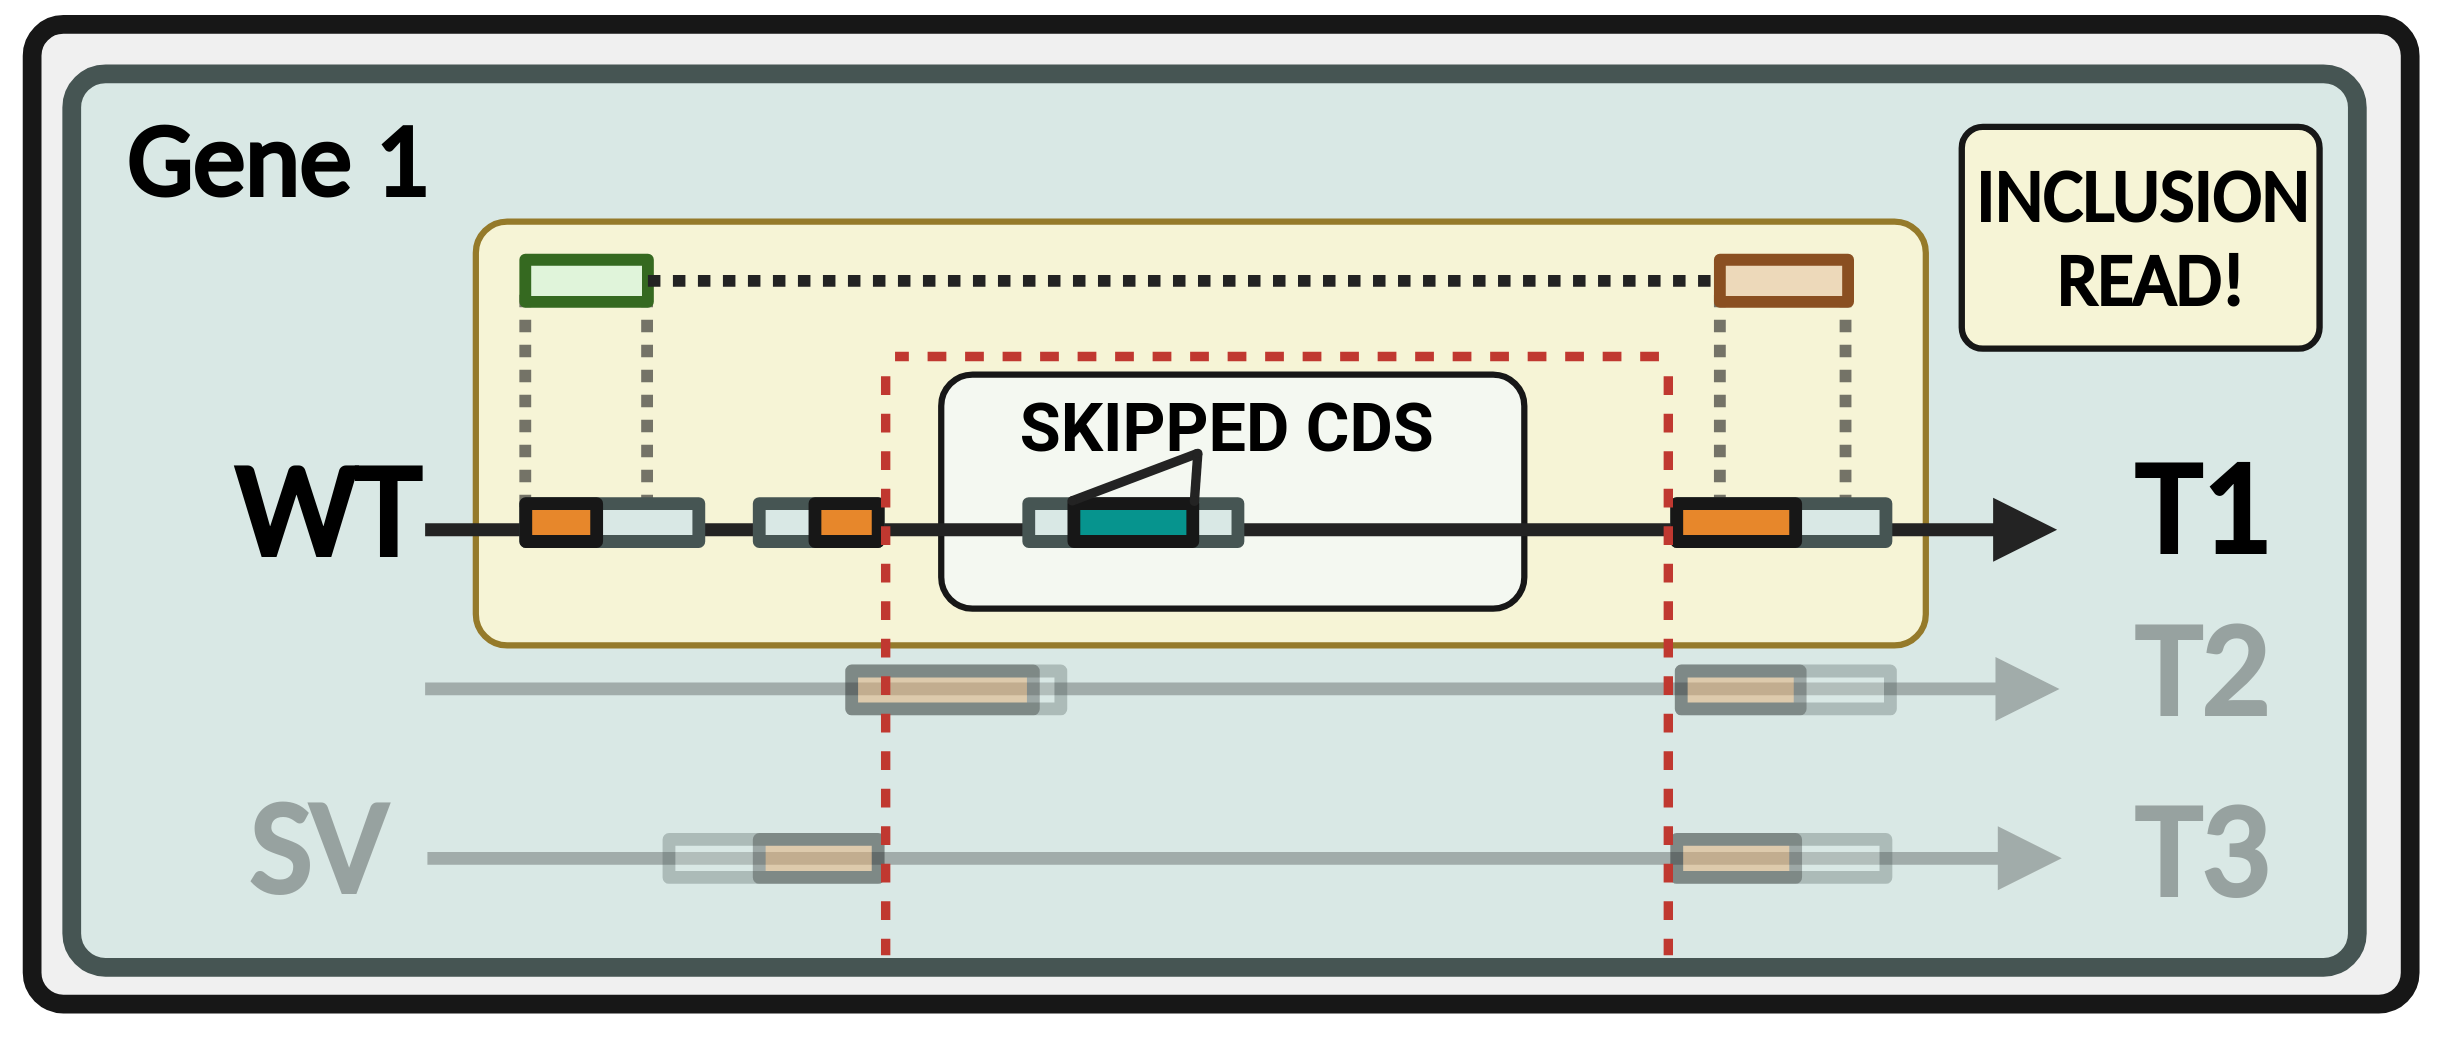
\includegraphics[width=0.8\textwidth]{./figures/EdgeCase.png}
    \caption{Sonderfall bei der Berechnung von \textit{ERC}. Der \textit{Read} passt hier nur auf \textbf{T1} und obwohl sich die übersprungene \textit{CDS} in der Lücke zwischen
    \textit{Forward} und \textit{Reverse Read} befindet, zählt dieser \textit{Read} als \textit{IRC}, denn er kann nur durch \textbf{T1} entstanden sein.
Die Abbildung wurde mit \cite{biorender} erstellt}
    \label{fig:-figures-EdgeCase-png}
\end{figure}

\section{Ergebnisse}\label{sec:Ergebnisse}
\subsection{PSI Werte}
\subsection{Vergleich mit DEXSeq}
\subsection{Laufzeit}
% ------------------------------------------------------------------------------





\newpage
% ------------------------------------------------------------------------------
\printbibliography
% ------------------------------------------------------------------------------


\end{document}
